\section{Merging Edited Packages}
\label{sec:merge}

\begin{figure}[H]
	\centering
	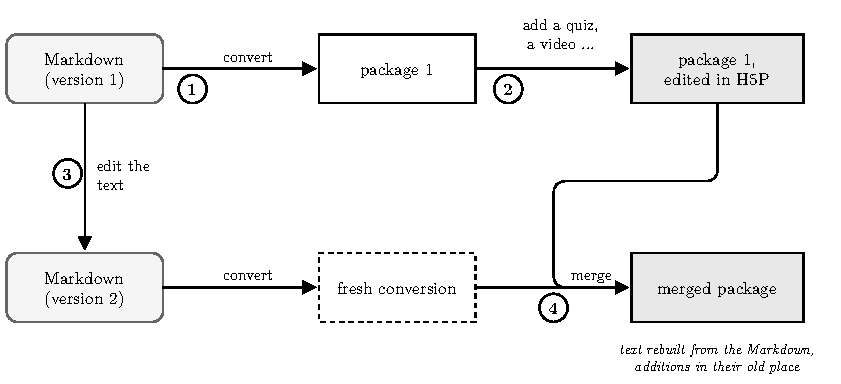
\includegraphics[width=0.95\columnwidth]{figures/merge-workflow}
	\caption[The editing cycle the merge exists for]{\label{fig:merge_workflow}The editing cycle the merge exists for.
	The Markdown is
		converted \circled{1}, the package is extended in the H5P editor \circled{2}, the Markdown
		changes \circled{3}, and the fresh conversion is merged with the edited package \circled{4}:
		the text is rebuilt from the Markdown, the additions keep their place.}
\end{figure}

The previous sections described a one-way conversion.
In practice, a teacher converts their notes, uploads the book, and then adds content in the H5P
editor that Markdown cannot express, such as a video, an image with hotspots, or a question type
that the question extension does not cover.
When the notes change later, a new conversion produces a package without these additions, and the
teacher would have to transfer them by hand.
\autoref{fig:merge_workflow} shows this cycle.
The converter therefore accepts the edited package as a second input \circled{4} to merge it with
the new conversion.

\subsection{Merge Policy}
\label{sec:mg_policy}

A three-way merge would have to reconcile the original Markdown, the revised Markdown, and the
edited H5P package.
If the same text is changed in both Markdown and H5P, the edits can conflict and require manual
resolution, as in a Git merge.
The converter avoids this complexity by preserving only additions from the H5P editor and dropping any edits to generated blocks, though warnings are issued for them.
The new Markdown conversion therefore replaces all generated blocks.
The remaining task is to place the manually added blocks among the newly generated blocks.

\subsection{Block Markers}
\label{sec:mg_markers}

For every block of the edited package, the merge has to know whether it came from Markdown or was manually added.
The package must therefore record the origin of its blocks in a form that survives an upload,
an editing session, and an export.

\begin{figure}[H]
	\centering
	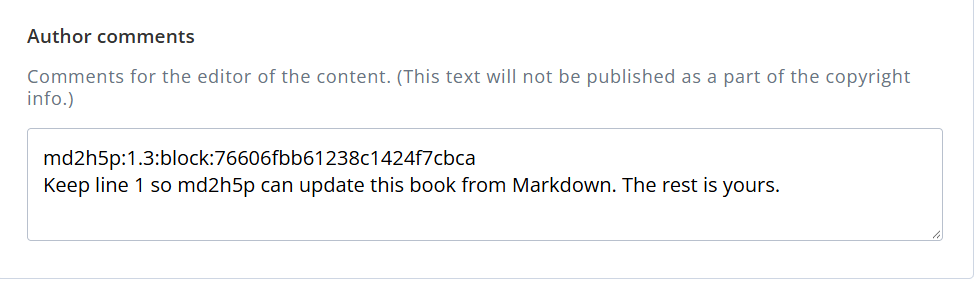
\includegraphics[width=0.9\columnwidth]{figures/screenshots/marker-comments}
	\caption[A marker in the metadata dialog of the H5P editor]{\label{fig:marker_dialog}The Author comments field
		of a generated block in the H5P editor's metadata dialog.}
\end{figure}

The converter records a marker in each generated chapter and top-level block, using the
\code{metadata.authorComments} field shown in \autoref{lst:marker}.
The first line contains a fixed prefix, the converter's version, the kind of element, and for a block
a hash of its content or for a chapter the name of its Markdown file.
The second line explains the purpose of the first one, since the field is visible to the teacher in
the metadata dialog of a block (\autoref{fig:marker_dialog}).

\par\medskip
\noindent\begin{minipage}{\linewidth}
\begin{lstlisting}[caption={[A block marker in \code{content.json}]A marker as it sits in \code{content.json}: the \code{authorComments}
field of one Text block, with the machine-readable first line and the explanation on the second.},
label={lst:marker}]
{
  "library": "H5P.AdvancedText 1.1",
  "params": { "text": "<p>The build has two stages, ...</p>" },
  "metadata": {
    "title": "Untitled Text",
    "authorComments": "md2h5p:1.3:block:18be0e19a4ab2eba443b37a2\nKeep line 1 so md2h5p can update this book from Markdown. The rest is yours."
  },
  "subContentId": "454e712b-26bd-aa20-f872-0941fa480cd8"
}
\end{lstlisting}
\end{minipage}

A marker alone suffices for identifying a block as generated from Markdown.
Unmarked blocks are consequently treated as manually added, even if their marker was deleted in the editor.
The marker's hash also detects changes to the block's content while ignoring metadata, whitespace
differences, and HTML tags to avoid reporting automatic editor changes.
Though changes to generated blocks can be detected and warned about through the hash, they cannot be reconciled under the chosen merge policy and are discarded.

\subsection{Alignment and Placement}
\label{sec:mg_alignment}

The additions must now be placed among the blocks of the new conversion.
An addition may have followed a paragraph that has since been reworded, split by an image, or deleted.
The merge therefore needs to recognize the corresponding block after its Markdown has changed.
Hashes alone cannot do this: even a typo correction changes the hash.

\paragraph{Block Similarity.}
An addition is anchored to the nearest preceding Markdown-generated block.
Consecutive additions are kept together in their original order.
Even if the anchor block has been reworded, it still likely resembles a block in the new conversion.
To find the counterpart and place the additions after it, the merge needs a measure of similarity.

The S{\o}rensen--Dice coefficient~\cite{Dice:1945} measures the overlap between two multisets.
Here, it is applied to adjacent word pairs extracted from the blocks' text.
Using word pairs rather than individual words makes the comparison stricter, since the words must
also occur next to each other in the same order to count toward similarity.
The coefficient divides twice the number of shared pair occurrences by the total number of pairs
in both texts.
Let $A$ and $B$ be the multisets of adjacent word pairs from two texts.
Their similarity is
\begin{equation}
    D(A,B) = \frac{2|A\cap B|}{|A|+|B|}.
    \label{eq:merge_dice}
\end{equation}
Here, $|A|$ and $|B|$ count word-pair occurrences; the intersection counts shared occurrences, including repetitions.
The result lies between 0 and 1, giving comparisons of different blocks a common scale.
A score of 0 means no shared pairs; 1 means identical pair counts, which does not necessarily imply
identical text.
\autoref{fig:merge_dice} gives a small example.

\begin{figure}[H]
    \centering
    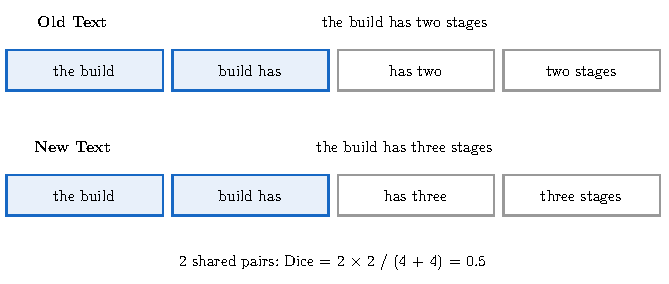
\includegraphics[width=\columnwidth]{figures/merge-dice}
    \caption[Similarity from adjacent word pairs]{\label{fig:merge_dice}Each text has four adjacent
        word pairs. Two pairs are shared (shaded), giving a similarity of $2\cdot2/(4+4)=0.5$.}
\end{figure}

Counting the word pairs in a hash table gives an expected running time of $O(m+n)$ for texts of
lengths $m$ and $n$.
This keeps each comparison inexpensive, which matters because every old block is compared with every new block.
Edit-distance measures are another option, but were not chosen because a standard Levenshtein
computation takes $O(mn)$ time for each comparison.

The text is taken only from the block's actual text, after removing all tags and metadata.
To prevent mix-ups between different kinds of blocks, two blocks of different libraries score 0.0, since a table or a question
never corresponds to a text block.

\paragraph{Alignment.}
Knowing how similar blocks are is not enough to place the additions.
Repeated passages may match several candidates, and a single old block may have been split into
several new ones.
The merge therefore needs a separate alignment algorithm to establish which blocks correspond.
The old and the new blocks of a chapter are aligned with the Needleman--Wunsch
algorithm~\cite{Needleman:1970}, a standard method for sequence alignment.
It considers block pairs with a S{\o}rensen--Dice score of at least 0.35 and finds the pairing with
the highest total score in which no two pairs cross.
This preserves the order of the blocks in the chapter.

\begin{figure}[H]
	\centering
	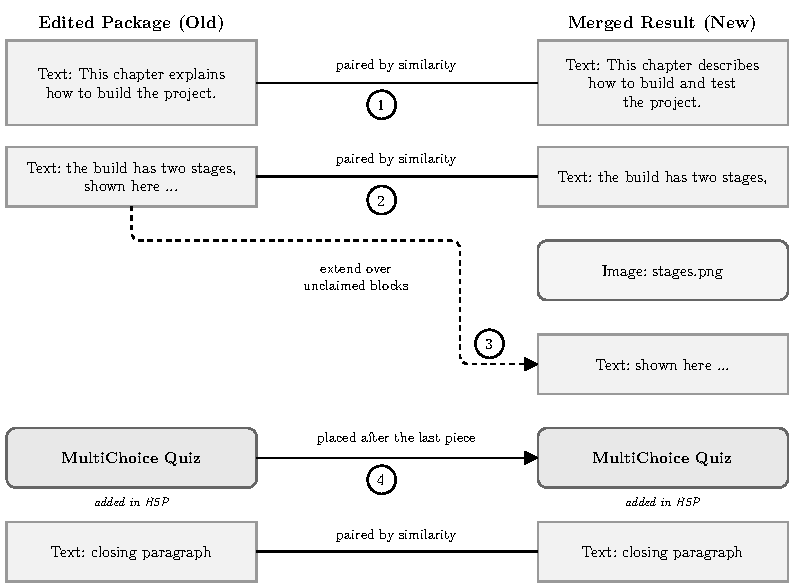
\includegraphics[width=\columnwidth]{figures/merge-alignment}
	\caption[Aligning the blocks of an edited chapter with the fresh conversion]{\label{fig:merge_alignment}Aligning the blocks of an edited chapter with the fresh
		conversion.
		Reworded blocks are paired by similarity \circled{1}~\circled{2}.
		A paragraph split by a new image is one old block and a run of new ones, so
		the anchor walks forward over the blocks nothing else claimed \circled{3}, and the quiz is
		placed after the last piece of the run \circled{4}.}
\end{figure}

\autoref{fig:merge_alignment} shows a chapter in which the introduction was reworded \circled{1}, a
paragraph was split by a new image \circled{2}, and a quiz had been added after that paragraph.
An addition remembers the block it followed and is placed after the block that one became
\circled{4}.

The split requires an additional step \circled{3}.
When an image is inserted into a run of paragraphs, the renderer emits text, image, and text where
there was a single Text block before.
One old block thus corresponds to a run of new blocks, and an addition that followed it
belongs after the last of them.
After the alignment, the merge scans the following unpaired blocks up to the first block paired
with another old block.
The anchor moves to the last of these blocks with a similarity of at least 0.15 to the old block.
Blocks in between, such as the new image, need not resemble it.
Conversely, if an image is removed, multiple blocks may become a single Text block.
The alignment in that case pairs one of the old text blocks with this combined block; the other old blocks
remain unpaired.

Two structural rules take precedence over the scores.
An addition at the very beginning stays first, and an addition that followed
the last block stays last, regardless of what the Markdown appends.
Only for a block that no longer exists does the merge have to guess.
It uses the nearest earlier block that still exists, then the nearest later one, and finally the end
or the beginning of the chapter, depending on which one is closer.
Only this case produces a warning.

This order-preserving alignment cannot represent a reordering.
If two paragraphs swap places in the Markdown, both cannot be paired correctly without crossings,
so a quiz added after one of them may end up after the wrong paragraph.
The text itself is not affected, since it is regenerated; only the additions may be misplaced.
The merge detects this case: if an old block scored strictly higher against a block it was not paired with, and the chapter
contains additions, the merge warns that the chapter appears to have been reordered.

\subsection{Chapters and Package Assembly}
\label{sec:mg_result}

\paragraph{Chapter Alignment.}
Changes to the Markdown source can also affect the naming or ordering of chapters.
To account for that, chapters are aligned in the same way, with a score determined in four steps.
Two chapters with the same source file name are the same chapter.
Otherwise, chapters with the same title are the same chapter.
Otherwise, the file names are compared after removing the number prefix and the extension and
normalizing punctuation, so that \code{3\_Retired.md} and
\code{03 - Retired.md} have the same name.
This step allows a book to be renumbered, which happens whenever a chapter is inserted in the middle.
Otherwise, the text of the chapters is compared like that of blocks.
This allows the merge to recognize the same chapter even if both its file name and its first heading
have changed.
A similar file name only adds a small bonus to the text score.
\code{3\_Basics.md} and \code{4\_Basics2.md}, for example, have very similar names but are two
different chapters.

\paragraph{Library Versions.}
A package names each library in three places that must agree: in the folder that contains it, in
the dependency list in \code{h5p.json}, and in the \code{library} field of every block.
A merge can bring them out of agreement because platforms upgrade their installed libraries, and a
package that was edited there may use newer versions.
For example, a generated book may use \code{H5P.Column 1.18}, while the edited package is automatically updated to use
\code{H5P.Column 1.22}.
Since mixing versions is not allowed by Moodle, the merged package needs to be updated to the versions of the edited package.
To do so, the merge keeps one version per library and rewrites every \code{library} field of the content accordingly.
However, the merge cannot run the migration scripts a library provides for a version change, so every version
change is reported in a warning.

\paragraph{Assembly.}
The result is built on the edited package rather than on the converter's template, so that the libraries
needed by the additions are included, even those the template does not contain.
The dependency lists of both packages are combined.
The media files must also be merged, so that media added both by the Markdown changes and
by the H5P changes sit alongside the existing ones.

With the merge, a book can be converted, extended in H5P, and converted again without losing these
additions.
